% ECE 412
% Forsman, Mejia-Rodriguez, Kulakevich, Wang

% Document settings ------------------------------------------------
\documentclass[a4paper,12pt]{article}

% Commands ------------------------------------------------
\newcommand{\authorname}{Forsman, Kulakevich, Mejia-Rodriguez, Wang}
\newcommand{\classnumber}{Capstone Group 10}
\newcommand{\projectname}{High Assurance Controller of Self-balancing Robot II}
\newcommand{\figHere}{\begin{overpic}[percent,scale=0.34]}	% Settings for all figures
\newcommand{\figHereB}{\begin{overpic}[percent,scale=0.5]}	% A different setting

% Packages ------------------------------------------------

\usepackage[USenglish]{babel} 	% American English
\usepackage{blindtext}			% Generate latin crap
\usepackage[yyyymmdd]{datetime} % Sets date format to ISO 8601 standard
\renewcommand{\dateseparator}{-}% Sets date format to ISO 8601 standard
\usepackage[nottoc]{tocbibind}  % References in TOC

\usepackage{graphicx}			% Image importing and display
\graphicspath{ {images/} }		% Path to image folder
\usepackage{xcolor}				% Allows normal color words
\usepackage{color, colortbl}

\usepackage{float}				% Adds 'H' for figure placement location
\usepackage{enumitem}			% Use for QandA environment
\usepackage{booktabs}			% Merging columns in tables
\usepackage{pdfpages}			% Add a PDF
\usepackage [autostyle, english = american]{csquotes}
\MakeOuterQuote{"}

\usepackage[nostamp]{draftwatermark}	% use [nostamp] when finished, [firstpage] otherwise
\SetWatermarkText{DRAFT}
\SetWatermarkColor{red!50}
\SetWatermarkScale{3}

\usepackage{overpic}				% Puts text over figures
\usepackage[american]{circuitikz}	% American-style circuit diagrams

\usepackage{amsmath}				% Multi-line equations
\usepackage{caption}				% Equation caption formatting
\usepackage{physics}				% Easier derivatives
\usepackage{gensymb}				% Enable \degree for degree symbol
\usepackage{siunitx}				% SI units
\usepackage[tablegrid]{vhistory}    % Version history

\usepackage{array}					% Used for centering tabular data
\newcolumntype{M}[1]{>{\centering\arraybackslash}p{#1}}  % The actual centered column format

\usepackage{listings} %For code in appendix

\definecolor{mymauve}{rgb}{0.58,0,0.82}
\definecolor{mygreen}{rgb}{0,0.6,0}
\definecolor{mygray}{rgb}{0.5,0.5,0.5}
\definecolor{ltgray}{rgb}{0.937, 0.937, 0.956}	% Divide standard RGB values by 255 for some reason 

% PSU colors
\definecolor{PSUgreen}{RGB}{106,127,16}
\definecolor{PSUltgreen}{RGB}{168,180,0}
\definecolor{PSUblue}{RGB}{0,117,154}
\definecolor{PSUltblue}{RGB}{161,216,224}
\definecolor{PSUgray}{RGB}{71,67,52}
\definecolor{PSUbrown}{RGB}{96,53,29}
\definecolor{PSUsienna}{RGB}{163,63,31}
\definecolor{PSUred}{RGB}{210,73,42}
\definecolor{PSUorange}{RGB}{220,155,50}
\definecolor{PSUyellow}{RGB}{230,220,143}
\definecolor{PSUtan}{RGB}{232,221,162}
\definecolor{PSUpurple}{RGB}{101,3,96}


\newenvironment{QandA}
	{\begin{enumerate}[label=\arabic*.]\sl} % Use slanted ques	tion text and Arabic numerals
  {\end{enumerate}}
\newenvironment{answered}{\par\normalfont}{} % Paragraph break and use normal font

% fancy header / footer lines
\usepackage{fancyhdr}% http://ctan.org/pkg/fancyhdr
\pagestyle{fancy}% Change page style to fancy
\fancyhf{}% Clear header/footer
\fancyhead[L]{\textcolor{PSUgray}{\classnumber}}
\fancyhead[R]{\textcolor{PSUgray}{\projectname}}
\fancyfoot[L]{\textcolor{PSUgray}{\authorname}}
\fancyfoot[R]{\textcolor{PSUgray}{\thepage}}
\renewcommand{\headrulewidth}{0.4pt}% Default \headrulewidth is 0.4pt
\renewcommand{\footrulewidth}{0.4pt}% Default \footrulewidth is 0pt


% Title Page ------------------------------------------------
\begin{document}
\lstset { %Formatting for code in appendix
  language=Matlab,
  basicstyle=\footnotesize\ttfamily,
  numbers=left,
  stepnumber=1,
  showstringspaces=false,
  tabsize=1,
  breaklines=true,
  breakatwhitespace=false,
  stringstyle=\color{mymauve},
  keywordstyle=\color{blue},
  commentstyle=\color{mygreen}, 
}

\begin{titlepage}
	\begin{center}
		\vspace*{1cm}

		\huge\textsc{\projectname}
		\vspace*{1cm}

		\textsc{Product Design Specification}

		\vspace{0.5cm}
		\small\textsc{\classnumber}
		
		\vspace{1.5cm}
		\normalsize \authorname 
		
		\vspace{0.5cm}
		%Lab TA: N/A
		
		\vfill
		\vspace{0.8cm}
		
		\includegraphics[width=0.5\textwidth]{images/psulogo_horiz_msword.tif}
		
		\vspace{0.5cm}
		Electrical and Computer Engineering\\
		Portland State University\\
		\today
		 
	\end{center}
\end{titlepage}
% Version History ------------------------------------------------
\begin{versionhistory}
    \vhEntry{0}{01/20/2020}{AF,IMR,AK,YW}{Initial Release}
    \vhEntry{1}{02/18/2020}{AF}{Added General Background and robot image citation}
    \renewcommand \vhAuthorColWidth{.8\hsize}
    \renewcommand \vhChangeColWidth{1.2\hsize}
\end{versionhistory}

% Table of contents ------------------------------------------------
\newpage
\tableofcontents 


% Begin paper ------------------------------------------------
\newpage
\pagenumbering{arabic}

\section{Introduction}
	The purpose of this document is to explain the requirements that Galois has given us in our project. In addition, we will communicate the background and research associated with several of the requirements. Specifically, we will provide information on the controller, firmware, verification, and robot design.
	
\section{Objective}
	Tools and practices for designing and verifying high assurance hardware/software systems are not fully standardized. High assurance systems are desirable in situations where a machine's performance could impact a person's health. In order to explore the processes involved in this type of development, a test case using a control system for a two-wheeled inverted pendulum (TWIP) will be explored and documented.
	
\section{General Background}
	A Two-Wheeled Inverted Pendulum is a type of robot that balances on two wheels. There are some clear advantages to this model (more stable up steep inclines, smaller footprint, fewer mechanical parts), however it is much less stable than four-wheeled robots. In order to keep the robot upright, a feedback system must be implemented. This system takes data describing the current position of the robot and translates it into motion in the wheels in order to prevent the robot from falling over. A PSU Capstone team from 2019 built such a robot and implemented a linear controller. In order to aid in this process, they also developed a model of the robot in MATLAB, and created a simulator that modeled the system's response to various inputs. Additionally, they did some work in exploring implementing the controller in Rust, a programming language that is designed to be inherently secure. This project intends to build on the work this previous team did, and continue some of the threads they began. 
	
	We will attempt to develop an alternative controller to the linear controller the previous team designed, using a model in MATLAB, verify that it works, and generate embedded Rust from verified code. Then the code will be loaded onto an upgraded robot, and it's performance compared with the model, as well as the previously implemented controller.
	
\section{Overview \& Guidelines}
The requirements have been broken into things that we “must” complete, “should” complete, and "may" complete. It should be noted that these requirements were set by Galois and may seem to be less abstract than normal.\\

\textbf{MUST}
\begin{itemize}
    \item Extend the existing code for the inverted pendulum robot to include a Rust control library.
    \item Modify Lustre/Kind 2 Rust code generator to generate “embedded-friendly” Rust, which can be directly imported in your library.
    \item Develop and identify a model of a nominal self-balancing robot in Octave or MATLAB.
    \item Isolate the “Software Under Test” as a severable block to analyze only the linear/non-linear controller for specific properties.
    \item Develop and identify a dynamics model of the robot in Octave or MATLAB.
    \item Develop and verify a controller with a wider range of stable input conditions and compare its performance with the PID controller through both simulation and in the real system.
    \item Build another robot with the upgraded parts provided by Galois.
\end{itemize}
\textbf{SHOULD}
\begin{itemize}
    \item Develop and verify a non-linear controller and compare its performance with the PID controller through both simulation and in the real system.
\end{itemize}
\textbf{MAY}
\begin{itemize}
    \item Attempt to leverage Rust Quickcheck to verify the properties developed in Kind 2 in the source files after the control design is implemented.
    \item Develop a suite of verified nonlinear controllers and compare their performance with linear variants.
    \item Translate Rust code into a LEAN theorem definitions for verification.
\end{itemize}

\section{Architecture Design}
\subsection{TWIP}
	\begin{figure}[H]
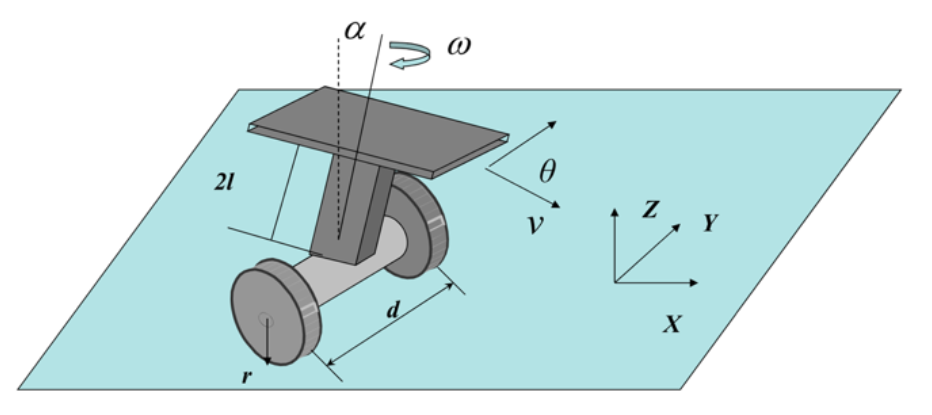
\includegraphics[width = \textwidth]{images/PDS_TWIP.png}
\caption{Simplified image of a TWIP\cite{yang}}
	\end{figure}
The model used for the design will be dependent upon the method of control that we wish to implement. For a linear control method the model will be centered about the equilibrium point corresponding to the two-wheeled inverted pendulum (TWIP) being upright. This yields the following state space representation \cite{yang} :
	\begin{figure}[H]
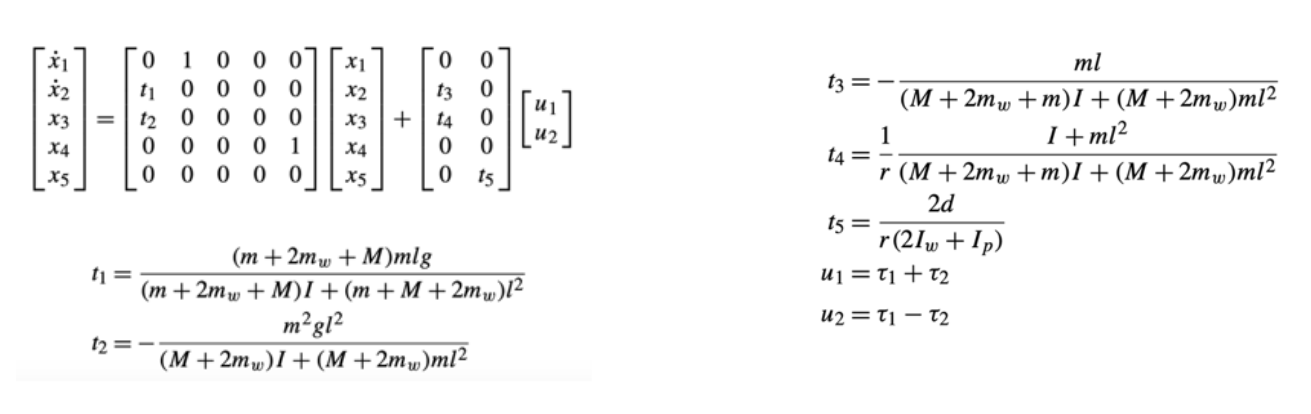
\includegraphics[width = \textwidth]{images/PDS_StateSpace.png}
\caption{Linearized state space representation of TWIP Dynamics \cite{yang}.}
	\end{figure}
Achieving a global model of the systems dynamics will be achieved as we make further progress in our project. 
\subsection{TWIP Controller}
As it stands, the dynamics of the two-wheeled inverted pendulum (TWIP) are represented by a linearized model. A linearized model can be achieved by using a Taylor series expansion around an equilibrium point \cite{yang}. Linearizing the system allows a designer to use a vast collection of well defined control techniques. However, when the system varies significantly from the equilibrium points, the controller is no longer effective. The need for a controller that can effectively stabilize the nonlinear dynamics of the system is evident. Prominent methods used to control nonlinear systems will be discussed below:
\subsubsection{Feedback linearization\cite{yang}}
This technique is essentially a way to cancel out the nonlinear dynamics of the system. Rather than doing so by approximation, this is done through a state transformation of the system. Once the feedback linearization is achieved all of the methods of linear controls can be used. This sounds advantageous, however it requires an exact knowledge of the system’s dynamics. Before implementing this method we would have to confirm that the dynamics model of the TWIP is accurate and precise. The basic block diagram for the feedback linearization loop is shown below: 
 \begin{figure}[H]
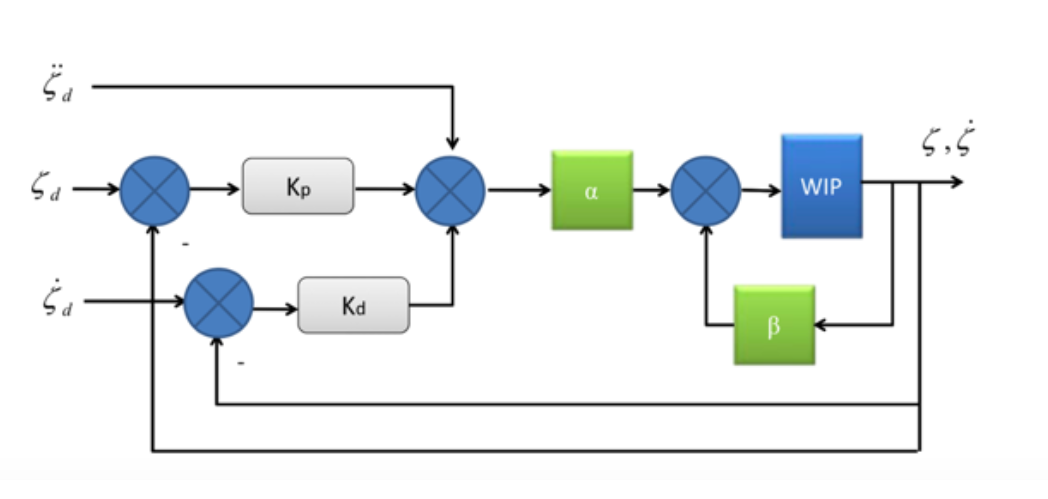
\includegraphics[width = \textwidth]{images/PDS_LinearFeedback.png}
\caption{Feedback linearized WIP with a Proportional plus derivative controller \cite{yang}.}
	\end{figure}
\subsubsection{Sliding mode control \cite{edwards}}
If an exact model of the dynamics associated with the TWIP cannot be obtained another suitable method of control must be implemented. One method is referred to as sliding mode control. This is a method where the control law is changed during process depending on the state of the system. The advantage of using this control method includes increased robustness (insensitivity to modeling errors) and operating range.
\subsubsection{Model Predictive Control \cite{brunton}}
Model predictive control is an online optimization method that allows the control signal to be continuously optimized based off of an established model. Implementing a nonlinear model may not be feasible if the hardware of the system does not permit fast enough computations. However, because of the continuous optimization it is possible to use a linearized model and achieve better specifications than an offline controller. In addition, constraints can be imposed on the control signal to keep the physical limitations of the actuators in consideration. This method relies on a good model of the system. A good model of the system can be achieved using machine learning techniques.
\subsection{Rust}
Rust is an evolving language that’s still in its early stages, it’s main aspects are performance, reliability, and productivity, with a strong emphasis on safety.  Rust was designed to compete with programming languages like C and C++, while adding features that are meant to make Rust safer than the other two languages.  Ownership and Lifetimes are two of the most important features exclusive to Rust. These are used to eliminate the need for garbage collection, and reduce the risk of a ‘data race’ (when two pointers access the same memory location at once), respectively.  Rust has a strict compiler that attempts to enforce ownership and lifetime rules before the code can go into runtime.  The goal is to make it significantly easier to catch  inconspicuous errors that often plague other lower level languages before the code ever leaves the compiler. \par
Another benefit of Rust is that the compiler is very helpful in describing possible issues and finding alternative solutions.  Additionally, the standard library provides many features that are borrowed from functional programming, some of which are shown in the figure below. Unfortunately, for our implementation we will be using Embedded Rust with our microprocessor that removes many of the features provided by the standard library: \par
 \begin{figure}[H]
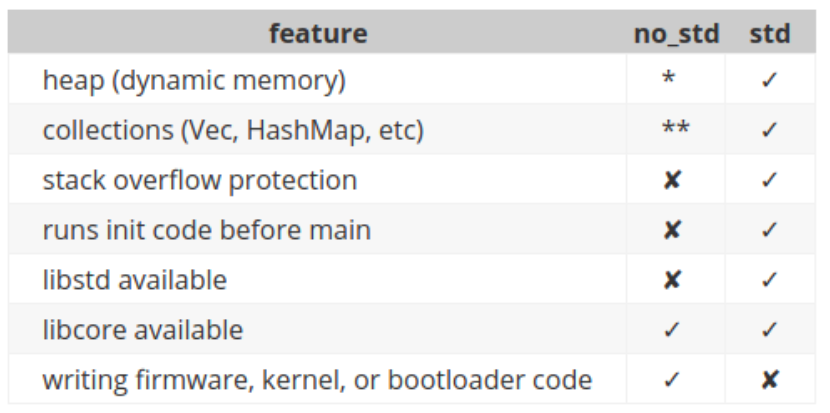
\includegraphics[width = \textwidth]{images/PDS_Rust.png}
\caption{std vs no-std feature overview \cite{greig}.}
	\end{figure}
Our required model verification tool Kind 2 has the option to compile Rust from Lustre, allowing for traceability between our model and our coded implementation.  This will allow us to generate Rust code that has properties that have been verified as invariant, and test it on our project without the risk for human error between the model we have created and code we have written for the robot. \par
Currently Kind 2 is not configured to generate “embedded-friendly” code, and one of our requirements will be to make Lustre to Rust “embedded-friendly” compilation an option.  This will require identifying the components of the Lustre to Rust compiler that introduces code not suitable for an embedded environment, and try to find alternatives in the core library or identify necessary limits on the Lustre code that will allow for embedded code generation. \par

Additional stretch goals have also been defined for our Rust implementation that user other features and external libraries that are available to Rust.  Cargo is a package manager for Rust that allows for easy distribution and documentation of Rust libraries, with a defined library layout.  One of our stretch goals is to implement a suite of Rust libraries, and following the Cargo documentation process will make it much easier to other to implement our code suite in other projects.
Other stretch goals include using Rust's Quickcheck feature to perform verification.
\subsection{Verification}
In order to ensure that the controller we have designed is what has been implemented into the Rust language, and that it will perform as we expect, we will need to use formal verification. We will use the method of model checking to achieve this goal. Model checking is a good candidate for this as model checking software is a mature area, and the software’s performance has been optimized.\cite{baier} \par
Model checking involves verifying properties of the model that are invariant. For our system, that would be something like for any input, our system remains stable. To do this in a systematic, traceable way, we will use the Kind 2 model checker, an SMT-based model checker. Kind 2 takes a Lustre (a programming language) file as an input and checks to see whether specified properties of the code are invariant for all inputs. If they are not invariant for all inputs, it reports the sequence(s) of inputs that result in the variance. \par

To get to point where we are checking that our controller is stable for all inputs, we will need to develop a model of both the robot’s hardware, as well as the controller, in Octave/MATLAB and then translate those models into Lustre code. Our general process will look something like this:
 \begin{figure}[H]
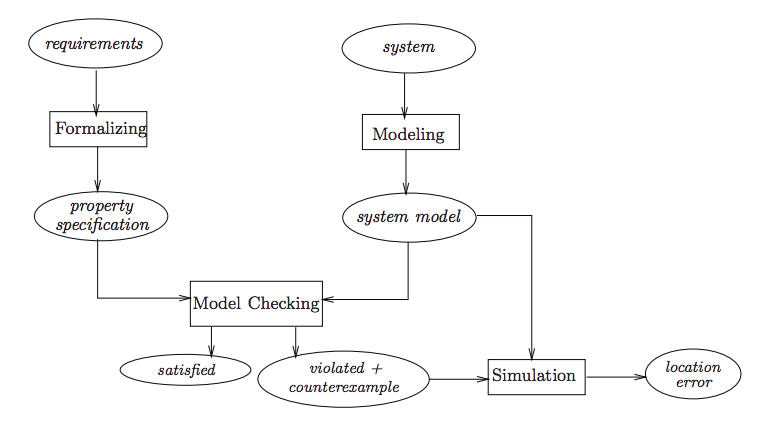
\includegraphics[width = \textwidth]{images/PDS_ModelChecker.png}
\caption{Model Checking Verification Process \cite{baier}.}
	\end{figure}
\par

As mentioned previously, we will use the Kind 2 model checker to generate Rust code that has been verified. By leveraging the model checker to produce Rust, we will be able to provide traceable, verifiable, stable, and safe code that should satisfy the "high-assurance" portion of this project's title.

\subsection{Robot}
There are many types of existing self-balancing robot structures. The structure shown in the figure below consists of three layers: the upper battery layer, the middle main control layer, and the bottom motor drive layer. The battery layer is used to place the 12V battery that powers the entire system. The main control layer consists of the minimum system of the main control chip and the sensor module. The motor drive layer receives the controller signals and controls the motor. Each layer is a functional module, and the circuit boards are supported and fixed between the layers. The motor shell is fixed to the motor drive circuit board. The motor shaft is connected to two tires.

 \begin{figure}[H]
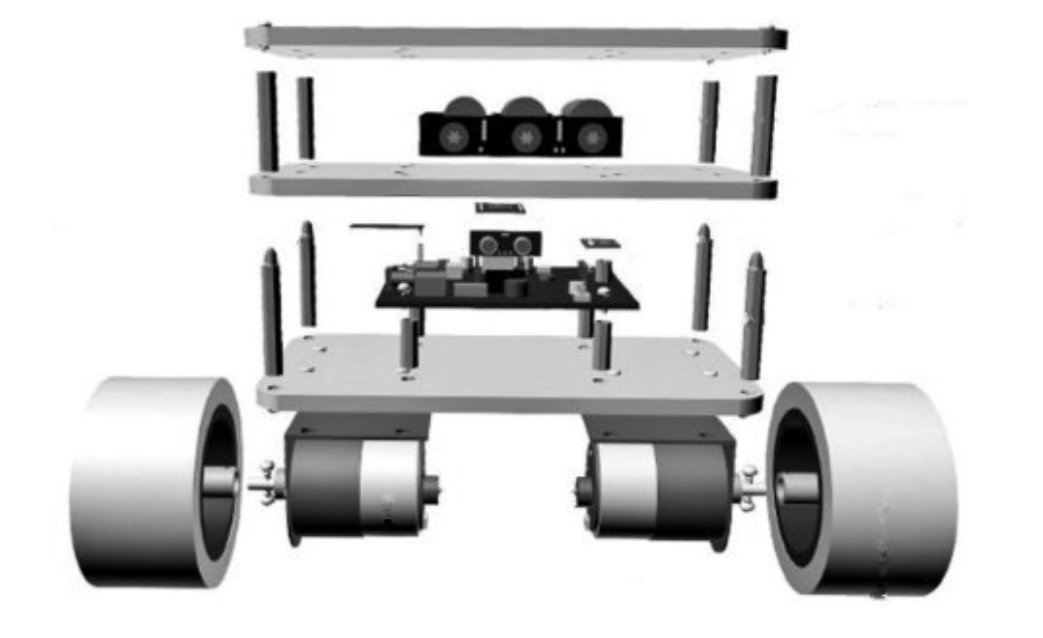
\includegraphics[width = \textwidth]{images/PDS_Robot.png}
\caption{Mechanical Structure of TWIP Robot.\cite{zhuqin}}
	\end{figure}
\par
The core problem of a two-wheeled balancing robot is the problem of motion balance control. Two-wheeled robots must always maintain an upright posture. While maintaining a balanced posture, they also need to complete various tasks, such as traveling, rotating, climbing, and crossing obstacles. The completion of these tasks will inevitably result in the elevation angle $\Theta$. Therefore, in order to balance the cart, the angle of elevation $\Theta$ must be reduced or even eliminated. In our design, we need to control $\Theta$ within a certain range. An effective method to eliminate the $\Theta$ angle is to use a feedback loop to engage the SAMD21 control motor, causing the chassis to move, ensuring that it is on the same vertical line as the upper and lower parts of the vehicle body.\par

Building on the last team's work, we will build a robot using parts provided by Galois. Since the last team's robot works fairly well already, we will be refining the design that they implemented, in order to provide a more stable version, hopefully making the controls and modeling portions of the project easier to achieve.

\newpage
\section{Approvals}
The undersigned acknowledge they have reviewed the Team 10 Product Design Specification document and agree with the approach it presents. Any changes to this Requirements Definition will be coordinated with and approved by the undersigned or their designated representatives.

\vspace{1cm}
\begin{tabular}{@{}p{.75in}p{4in}@{}}
Signature: & \hrulefill \\
Print: & \hrulefill \\
Title: & \hrulefill \\
Date: & \hrulefill \\
\end{tabular}

\vspace{1cm}
\begin{tabular}{@{}p{.75in}p{4in}@{}}
Signature: & \hrulefill \\
Print: & \hrulefill \\
Title: & \hrulefill \\
Date: & \hrulefill \\
\end{tabular}

\vspace{1cm}
\begin{tabular}{@{}p{.75in}p{4in}@{}}
Signature: & \hrulefill \\
Print: & \hrulefill \\
Title: & \hrulefill \\
Date: & \hrulefill \\
\end{tabular}

\newpage
\bibliographystyle{unsrt}
\bibliography{ref}
\end{document}
